\chapter{Conditional diffusion models} \label{ch:conditional-diffusion}

So far we have described diffusion models as models that can be fit to describe a single distribution. In this chapter we introduce and motivate conditional diffusion models as well as conditional generative models more broadly. A conditional generative model is trained on paired data $\rvx, \rvy \sim p_\text{data}(\cdot, \cdot)$ and then, at test-time, can be given $\rvy$ as an input and produces samples from an approximation of the conditional distribution $p_\text{data}(\rvx|\rvy)$. Conditional generative models have applications in text-to-image systems (\cref{fig:dalle-3-samples}), image editing tools (\cref{fig:emu-edit-samples}), and more domains. Additionally, as we will discuss in \cref{sec:conditioning-on-more-improves-performance}, conditional diffusion models can often generate more realistic samples than unconditional diffusion models. Developing conditional diffusion models can therefore be useful even if the task of interest is to model a single distribution without conditioning. Before motivating the use of conditional diffusion models further, we will transport the important results of \cref{ch:diffusion} from the unconditional to the conditional diffusion modelling setting in \cref{sec:conditional-diffusion-overview}.

\begin{figure}[t]
    \centering
    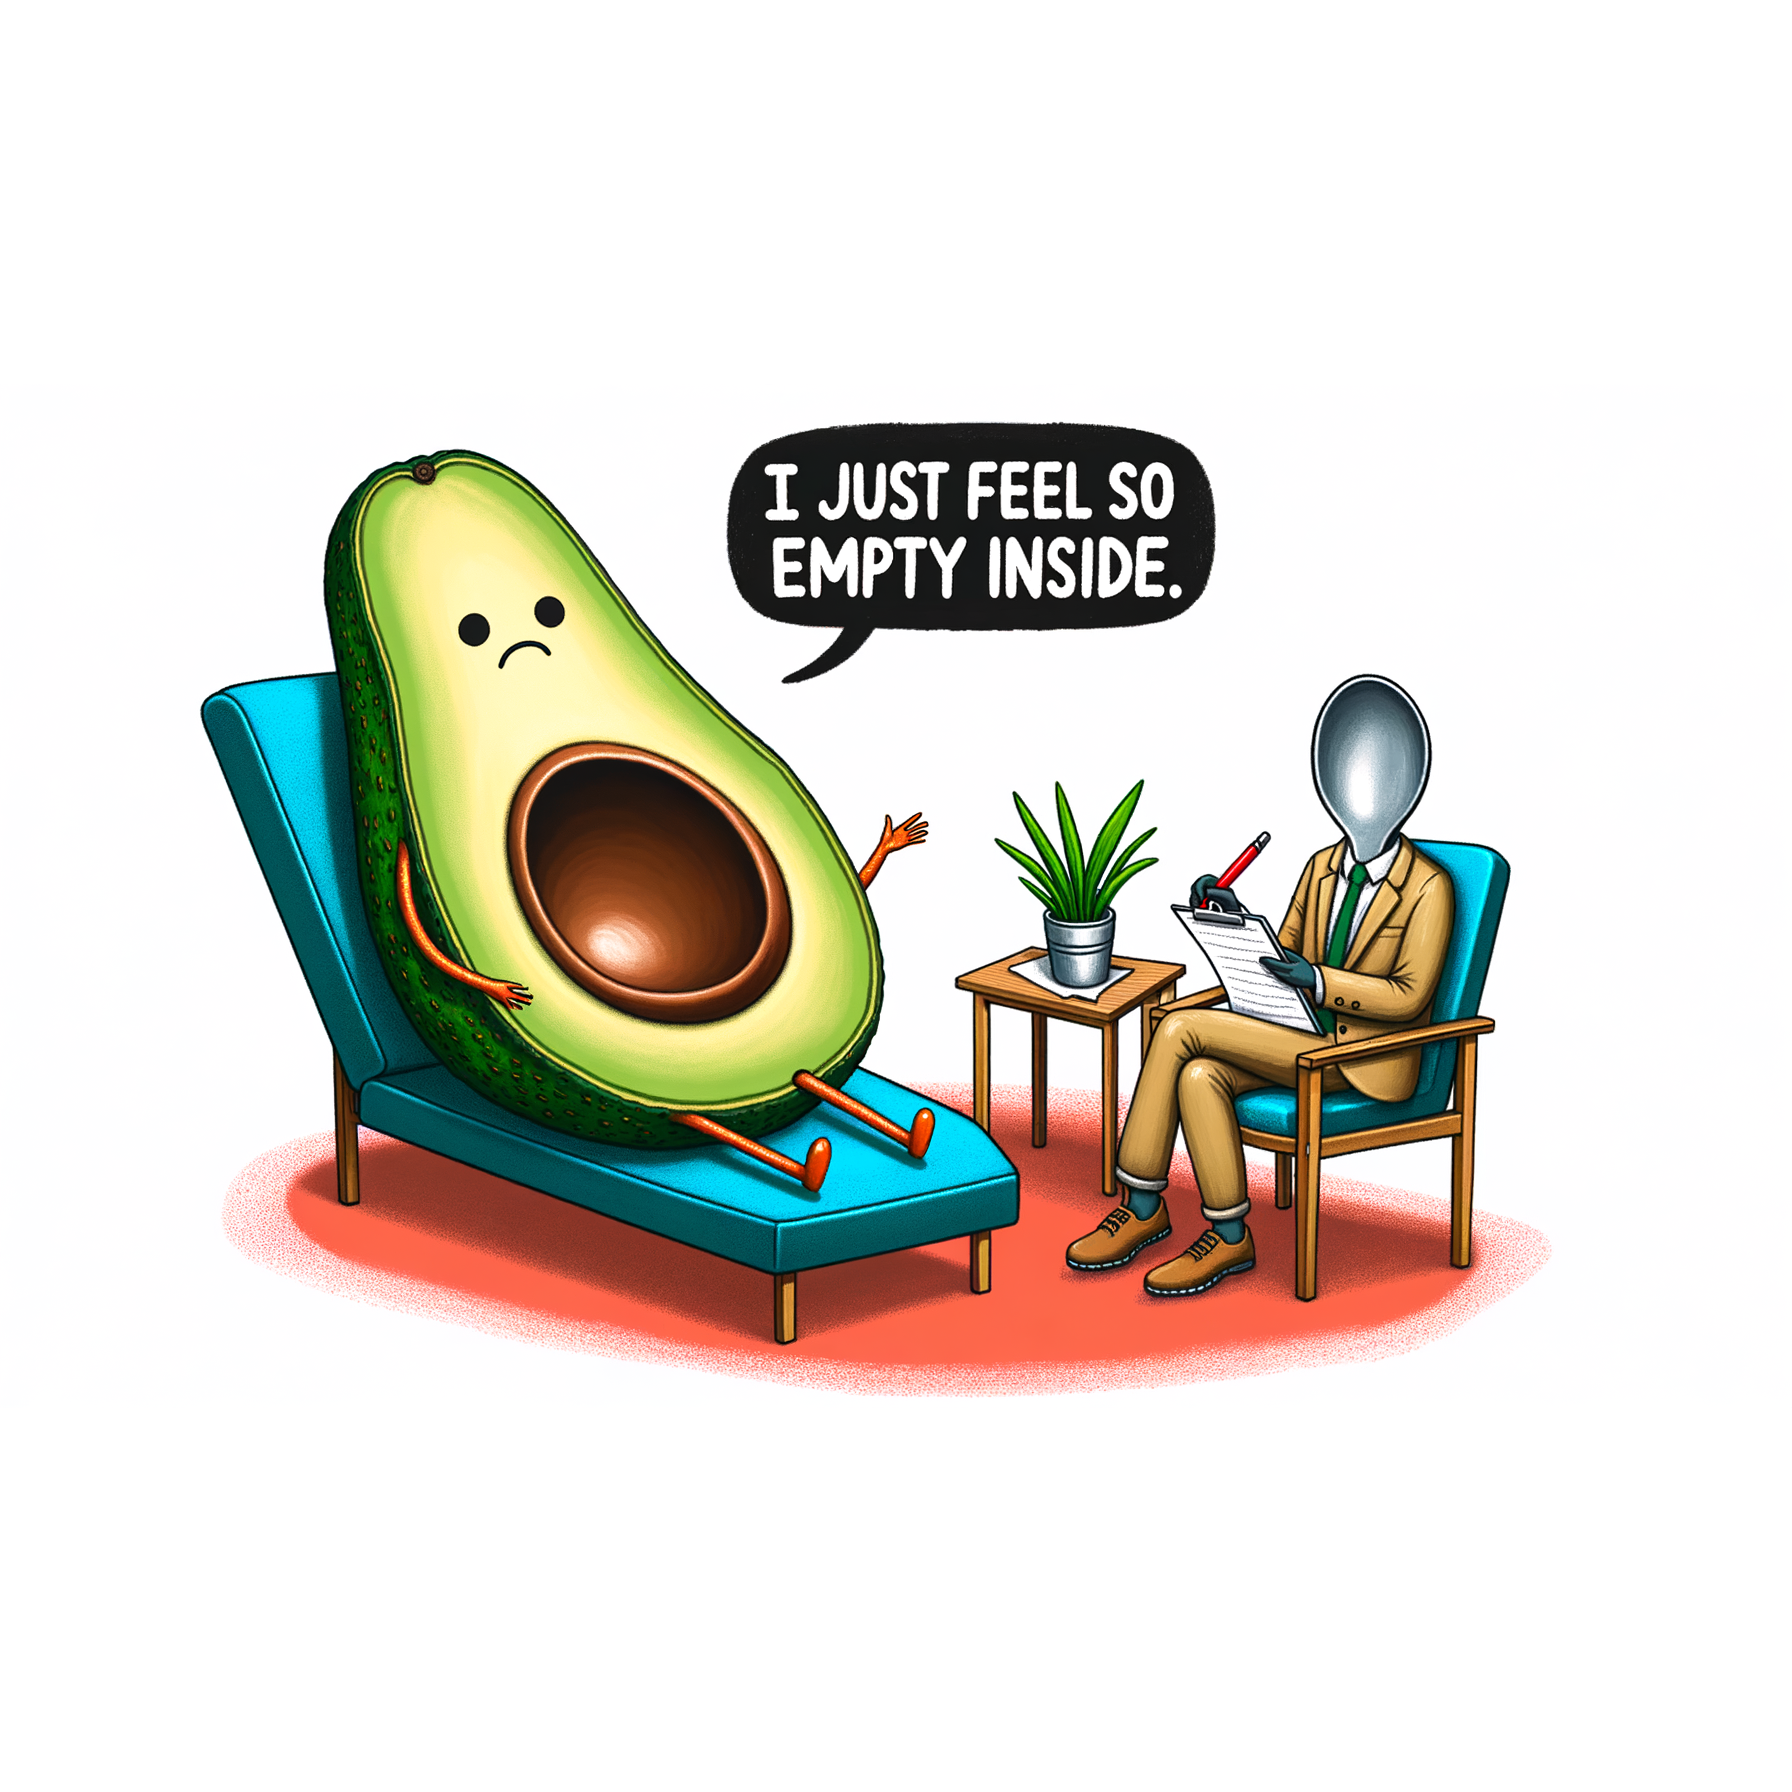
\includegraphics[width=0.32\textwidth]{figs/thesis/dalle3/1.png}
    \hfill
    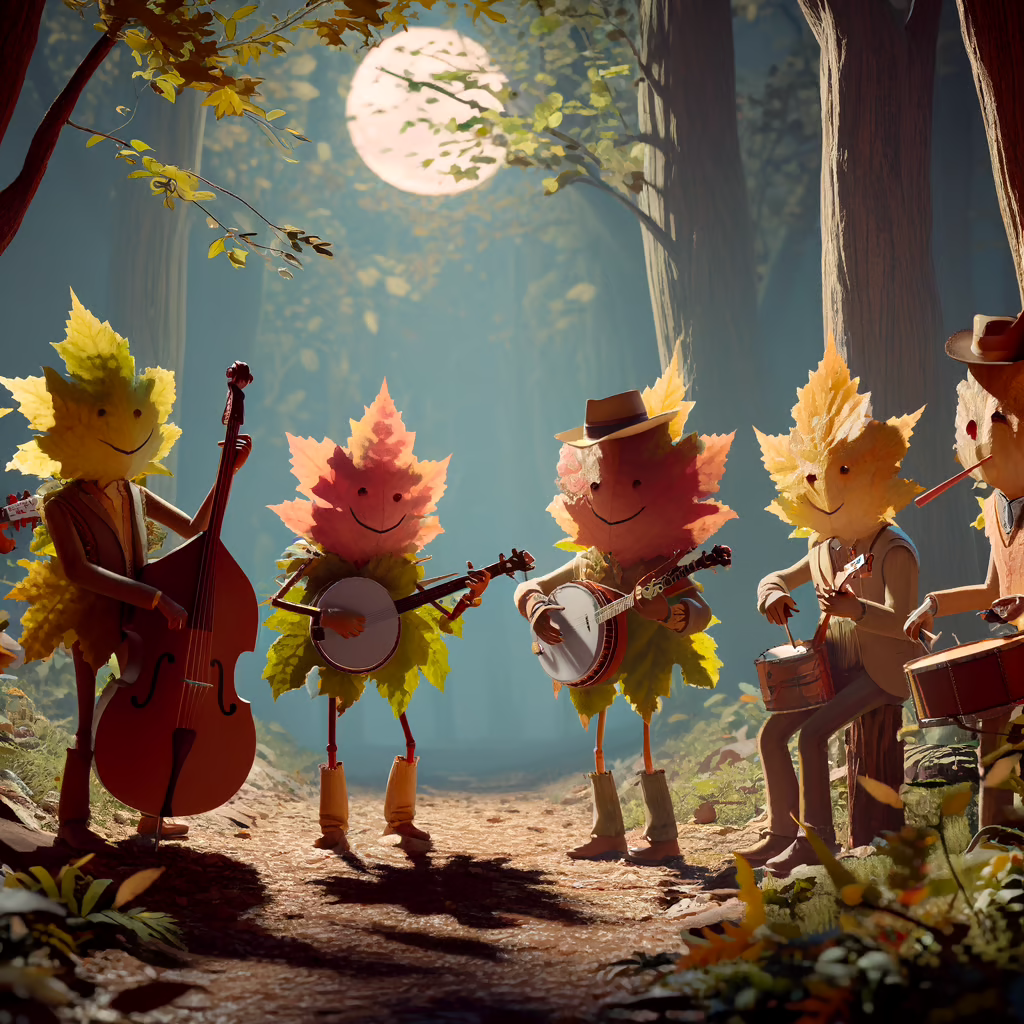
\includegraphics[width=0.32\textwidth]{figs/thesis/dalle3/2.png}
    \hfill
    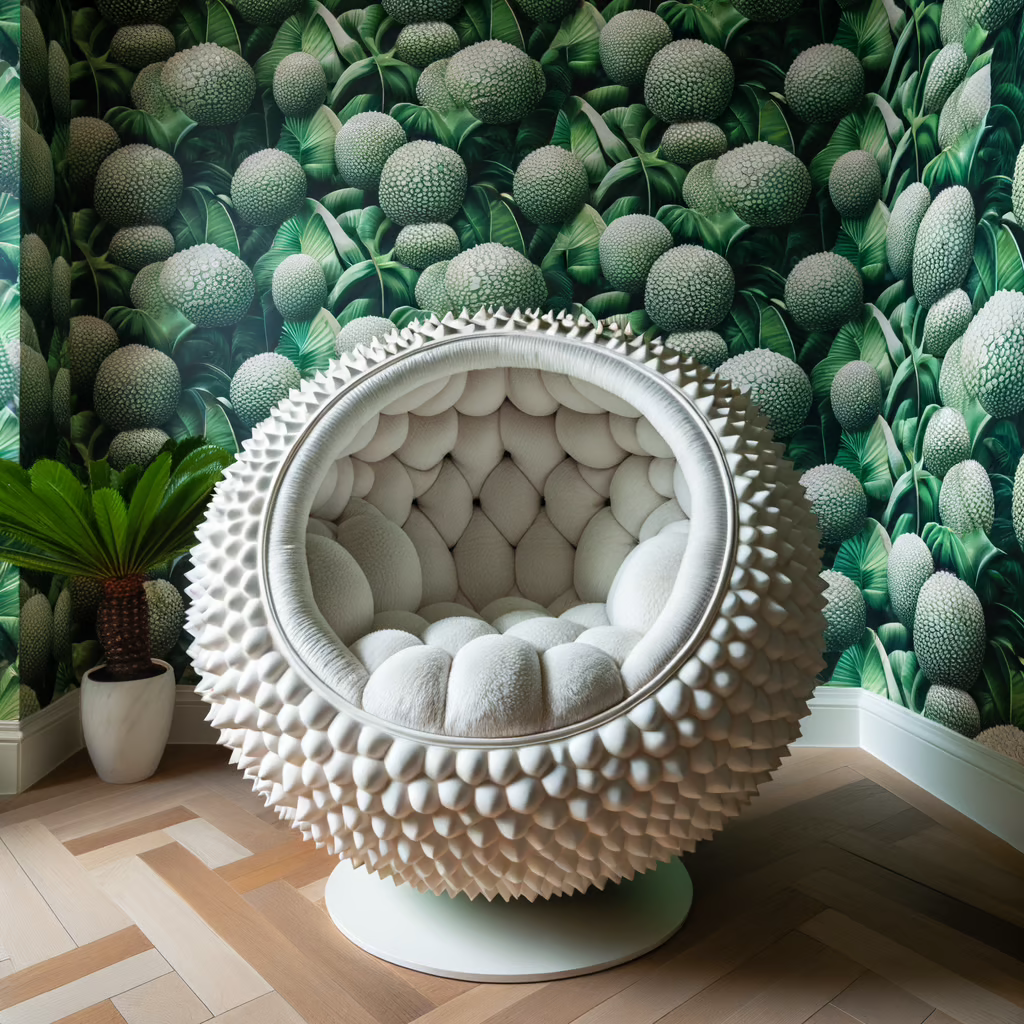
\includegraphics[width=0.32\textwidth]{figs/thesis/dalle3/4.png}
    \caption{Images sampled by diffusion model DALL-E 3~\citep{betker2023improving} given text prompts, from left to right, ``An illustration of an avocado sitting in a therapist's chair, saying 'I just feel so empty inside' with a pit-sized hole in its center. The therapist, a spoon, scribbles notes.''; ``A 2D animation of a folk music band composed of anthropomorphic autumn leaves, each playing traditional bluegrass instruments, amidst a rustic forest setting dappled with the soft light of a harvest moon.''; and ``Photo of a lychee-inspired spherical chair, with a bumpy white exterior and plush interior, set against a tropical wallpaper.''. Reprinted with permission of \citeauthor{betker2023improving}.}
    \label{fig:dalle-3-samples}
    \centering
    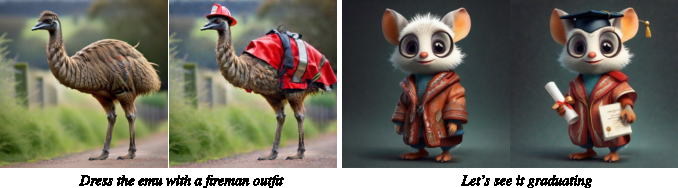
\includegraphics{figs/thesis/emu_edit_examples.pdf}
    \caption{Image edits by a conditional diffusion model, Emu Edit~\citep{sheynin2023emu}. Given an input image (left of each pair) and text prompt, Emu Edit samples an edited image (right of each pair). Reprinted with permission of \citeauthor{sheynin2023emu}.}
    \label{fig:emu-edit-samples}
\end{figure}

\section{Introduction to conditional diffusion models} \label{sec:conditional-diffusion-overview}

In this section we restate the main results from \cref{ch:diffusion} in the conditional diffusion modelling setting. In this setting we will assume that there is a data distribution $p_\text{data}(\rvx, \rvy)$ and we can access $(\rvx, \rvy)$ pairs sampled from it to train our model. Our objective will be to train a model which, given any value of the \textit{conditioning information} $\rvy$, can return a good approximation of the conditional distribution $p_\text{data}(\rvx|\rvy)$, which according to Bayes' rule is equal to $\frac{p_\text{data}(\rvx,\rvy)}{\int p_\text{data}(\rvx,\rvy) \mathrm{d}\rvx}$. The conditioning information can take the form of, for example, an image, a text prompt, a class label, and embedding vector, or a combination of multiple such items.

\paragraph{Training a conditional diffusion model}
To use the methodology from \cref{ch:diffusion} in this setting, we can imagine simply training a different unconditional diffusion model for every possible value of $\rvy$. To do so, we could express the parameters as $\theta[\rvy]$, letting $\theta$ be a data structure that maps from any conditioning information $\rvy$ to the relevant set of diffusion model parameters. Then we could rewrite the diffusion model loss in \cref{eq:general-dm-loss} for a given $\rvy$ as
\begin{align} \label{eq:cond-diffusion-loss-single-y}
    \gL_\text{CDM}(\theta, \rvy) &= \EX_{u(t)q(\rvx_t|\rvx)\pdata(\rvx|\rvy)} \left[ \frac{\lambda^\rvs(t)}{u(t)} 
    || \rvs_{\theta[\rvy]}(\rvx_t, t) - \frac{\alpha(t)\rvx-\rvx_t}{\sigma(t)^2} ||_2^2 \right]
\end{align}
where we use $\theta[\rvy]$ in place of $\theta$ and sample $\rvx$ from $\pdata(\rvx|\rvy)$ instead of $\rvy$. To train the parameters for all $\rvy$ we may take an expectation of this loss over $\rvy$:
\begin{align} \label{eq:cond-exp-diffusion-loss-all-sigma}
    \gL_\text{CDM}(\theta) &= \EX_{\pdata(\rvy)} \left[ \gL_\text{CDM}(\theta, \rvy) \right] \\
    &= \EX_{u(t)q(\rvx_t|\rvx)\pdata(\rvx, \rvy)} \left[ \frac{\lambda^\rvs(t)}{u(t)} 
    || \rvs_{\theta[\rvy]}(\rvx_t, t) - \frac{\alpha(t)\rvx-\rvx_t}{\sigma(t)^2} ||_2^2 \right].
\end{align}
This objective is feasible to use if $\rvy$ is discrete and has sufficiently few possible values but if not then it will be inefficient or impossible to train a different set of parameters $\theta[\rvy]$ for every possible value of $\rvy$.

A solution is to share parameters between the score functions used for different $\rvy$. A standard way to do so is to use the same parameters $\theta$ for each, but pass $\rvy$ as an additional input into the function~\citep{sohn2015learning}. The learned score function $\rvs_\theta(\cdot, \rvy, t)$ may then depend on $\rvy$ in an arbitrarily complex way (thanks to the universal approximation theorem~\citep{hornik1989multilayer}) while still being able to share information between different values of $\rvy$ using the single shared set of neural network parameters $\theta$. We will from now on write the learned score function for a conditional diffusion model as $\rvs_\theta(\rvx_t, \rvy, t)$. For brevity, we will also expand the definition of the joint distribution $q$ to include $\rvy$ as $q(\rvx,\rvy,\rvx_{t_1},\ldots,\rvx_{t_n}) := q(\rvx_{t_1},\ldots,\rvx_{t_n}|\rvx,\rvy)\pdata(\rvx,\rvy)$ so the training objective becomes
\begin{align} \label{eq:cond-diffusion-loss}
    \gL_\text{CDM}(\theta) &= \EX_{u(t)q(\rvx_t, \rvx, \rvy)} \left[ \frac{\lambda^\rvs(t)}{u(t)} 
    || \rvs_{\theta}(\rvx_t, \rvy, t) - \frac{\alpha(t)\rvx-\rvx_t}{\sigma(t)^2} ||_2^2 \right].
\end{align}
We will similarly write the learned predictions of $\rvx$ and $\epsilon$ as $\hat{\rvx}_{\theta}(\rvx_t, \rvy, t)$ and $\hat{\mathbf{\epsilon}}_{\theta}(\rvx_t, \rvy, t)$ respectively.
Based on \cref{eq:cond-diffusion-loss-single-y} it is clear that, given some $\rvy$, the diffusion model is learning an approximation of $\pdata(\rvx|\rvy)$. We will therefore denote the distribution it parameterises $p_\theta(\rvx|\rvy)$.

\paragraph{Sampling from a conditional diffusion model}
Other than the new input of $\rvy$, the sampling procedure remains the same. To be explicit, we will nevertheless restate the reverse SDE from \cref{eq:diffusion-edm-sde-approx} in the conditional case:
\begin{align}
    \mathrm{d}\rvx_t = \underbrace{- \frac{1}{2} g(t)^2 \rvs_\theta(\rvx_t, \rvy, t) \mathrm{d}t}_{\shortstack{\footnotesize Diffusion ODE \\ \footnotesize similar to \cref{eq:diffusion-ode}}} - \underbrace{\beta(t) \sigma(t)^2 \rvs_\theta(\rvx_t, \rvy, t) \mathrm{d}t + \sqrt{2\beta(t)}\sigma(t)\mathrm{d}\bar{\rvw}}_\text{\footnotesize Langevin diffusion}.
\end{align}
The only difference from \cref{ch:diffusion} is that there is an additional input of $\rvy$ to $\rvs_\theta$. Recall that this SDE becomes the reverse diffusion ODE from \cref{sec:diffusion-ode} when $\beta(t) = 0$ or the standard reverse diffusion SDE from \cref{sec:diffusion-reverse-sde} when $\beta(t) = \frac{g(t)^2}{2 \sigma(t)^2}$.

\paragraph{Computing likelihoods for conditional diffusion models}
It is possible to compute data likelihoods $p_\theta(\rvx|\rvy)$, or to weight the training objective to lower-bound this likelihood, similarly to the techniques described in \cref{ch:diffusion}. We do not present these results as this is not a focus of this dissertation.

\section{Conditioning on more information improves sample quality} \label{sec:conditioning-on-more-improves-performance}

So far we have mentioned the types of new applications that conditional diffusion models enable as well as introducing the conditional diffusion modelling framework. In this section we make the case that building conditional diffusion models is useful even if the task of interest involves modelling only a single unconditional distribution. We do so by showing that, at least in the image domain, conditional diffusion models often achieve better sample quality than unconditional diffusion models, and then that this insight can be used to make improved \textit{unconditional} generative models that incorporate \textit{conditional} diffusion models.

The better realism of samples from conditional DMs versus unconditional DMs has previously been noted by \citet{ho2022classifier,bao2022conditional,hu2022self}. Conditional DMs have also been observed to work better with few sampling steps~\citep{meng2022distillation}. Furthermore, we will show that sample realism grows with ``how much'' information the DM is conditioned on. To better make this point, we will distinguish between ``strongly-conditional'' generation, where we condition on a high-dimensional feature like a long text prompt, and ``lightly-conditional'' generation, where we condition on a lower dimensional feature like a class label or short text prompt.  As hinted at in \cref{fig:stable-diffusion-example} an image is likely to be more realistic if conditioned on being ``an aerial photograph of a road between green fields'' (strongly-conditional generation) than if it is if simply conditioned on being ``an aerial photograph'' (lightly-conditional generation). Unconditional generation of images will typically lead to even less realism.

\begin{figure}[t]
    \centering
    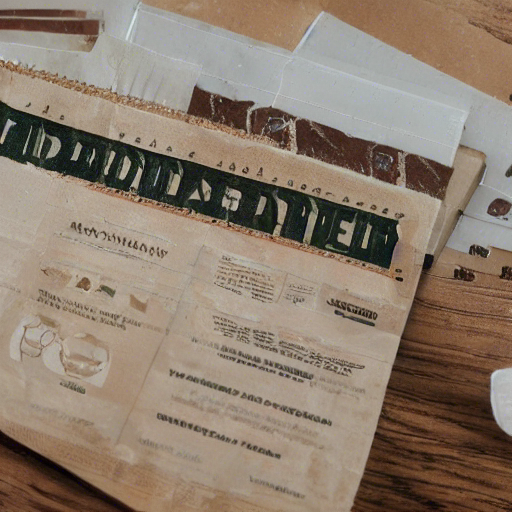
\includegraphics[width=0.3\textwidth]{figs/2sdm/sd_uncond.png}
    \hfill
    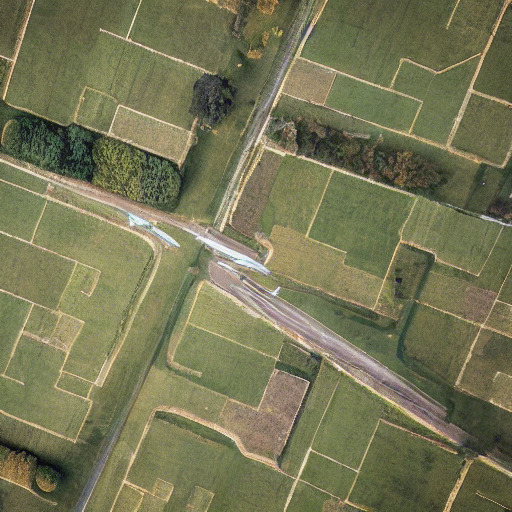
\includegraphics[width=0.3\textwidth]{figs/2sdm/uncond-aerial-photo.jpg}
    \hfill
    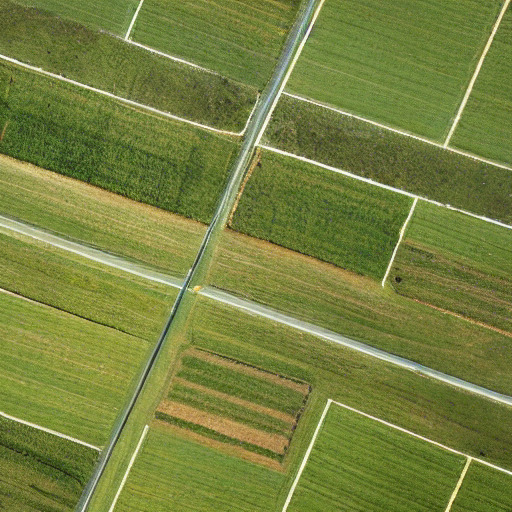
\includegraphics[width=0.3\textwidth]{figs/2sdm/cond-aerial-photo.jpg}
    \caption{Images sampled by Stable Diffusion~\citep{rombach2022high} with the same random seed and three text prompts. \textbf{Left:} Output with an empty text prompt. \textbf{Centre:} Output when prompted to produce ``aerial photography''. \textbf{Right:} Output given a more detailed prompt\protect\footnotemark. Using the more detailed prompt removes the ``smudged'' road artefact visible in the centre image.}
    \label{fig:stable-diffusion-example}
\end{figure}
\footnotetext{We used the prompt ``Aerial photography of a patchwork of small green fields separated by brown dirt tracks between them. A large tarmac road passes through the scene from left to right.''}

\subsection{Analysing conditional vs unconditional DMs} \label{sec:2sdm-cond-vs-uncond-dgms}

We will investigate the phenomenon of conditional DMs outperforming unconditional DMs primarily in the context of conditioning on CLIP (contrastive language-image pre-training)~\citep{radford2021learning} image embeddings. These are embedding vectors encoding high-level, semantically-meaningful information about a given image. The training procedure for such an image embedder is as follows. CLIP jointly trains two neural networks, an image embedder $e_i(\cdot)$ and a text embedder $e_t(\cdot)$, on a large captioned-image dataset. Given an image $\rvx$ and a caption $\rvy$, the training objective encourages the cosine similarity between $e_i(\rvx)$ and $e_t(\rvy)$ to be large if $\rvx$ and $\rvy$ are a matching image-caption pair and small if not.
The image embedder therefore learns to map from an image to a semantically-meaningful embedding capturing any features that may be included in a caption. We use a CLIP image embedder with the ViT-B/32 architecture and weights released by \citet{radford2021learning}. We can visualise the information captured by the CLIP embedding by showing the distribution of images produced by our conditional DM given a single CLIP embedding; see \cref{fig:samples}.

\paragraph{What does it mean to say that conditional DMs beat unconditional DMs?} A standard procedure to evaluate unconditional DMs is to start by sampling a set of $N$ images independently from the model: ${\rvx^{(1)},\ldots,\rvx^{(N)} \sim p_\theta(\cdot)}$. We can then compute the Fr\'echet Inception distance (FID)~\citep{heusel2017gans} between this set and the dataset. If the generative model matches the data distribution well, the FID will be low.
%
For conditional DMs the standard procedure has one extra step: we first independently sample ${\rvy^{(1)},\ldots,\rvy^{(N)} \sim \pdata(\cdot)}$. We then sample each image given the corresponding $\rvy^{(i)}$ as ${\rvx^{(i)} \sim p_\theta(\cdot|\rvy^{(i)})}$. 
%
Then, as in the unconditional case, we compute the FID between the set of images $\rvx^{(1)},\ldots,\rvx^{(N)}$ and the dataset, without reference to $\rvy^{(1)},\ldots,\rvy^{(N)}$. Even though it does not measure alignment between $\rvx, \rvy$ pairs, conditional DMs beat comparable unconditional DMs on this metric in many settings: class-conditional CIFAR-10 generation~\citep{karras2022elucidating}, segmentation-conditional generation~\citep{hu2022self}, or bounding box-conditional generation~\citep{hu2022self}.

\begin{figure}[t]
    \centering
    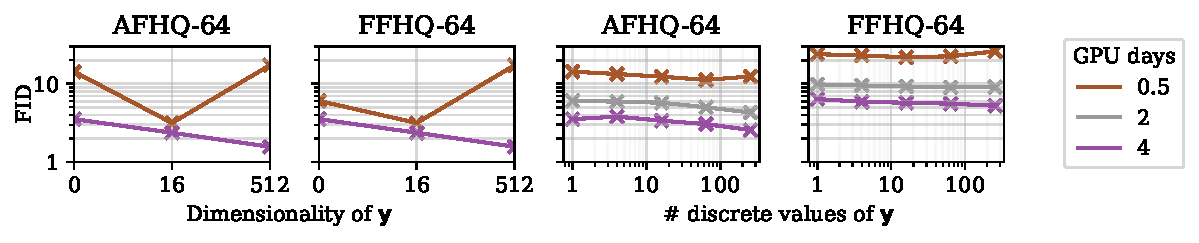
\includegraphics[width=\textwidth]{figs/2sdm/cond-results-vs-nclusters.pdf}
    \caption{Sample quality (measured by FID) versus the dimensionality of conditioning information $\rvy$ for CLIP-conditional image diffusion models on AFHQ~\citep{choi2020stargan} and FFHQ~\citep{karras2018style}. With small training budgets (brown line), it is harmful when $\rvy$ is too informative. With larger training budgets (purple line), it is helpful to make $\rvy$ much more high dimensional.}
    \label{fig:fid-vs-ncomp}
\end{figure}

\paragraph{Why do conditional DMs beat unconditional DMs?}

Conditional DMs ``see'' more data during training than their unconditional counterparts because updates involve $\rvy$ as well as $\rvx$. \citet{bao2022conditional,hu2022self} prove that this is not the sole reason for their successes because the effect holds up even when $\rvy$ is derived from an unconditional dataset through self-supervised learning.
%
To our knowledge, the best explanation for their success is, as stated by \citet{bao2022conditional}, that conditional distributions typically have ``fewer modes and [are] easier to fit than the original data distribution.''

\paragraph{When do conditional DMs beat unconditional DMs?}
%
We present results in \cref{fig:fid-vs-ncomp} to answer this question. We show FID scores for conditional DMs trained to condition on embeddings of varying information content. 
%
We produce $\rvy$ by starting from the CLIP embedding of each image in our dataset and using either principal component analysis to reduce their dimensionality (left two panels) or K-means clustering to discretize them (right two panels)~\citep{hu2022self}.
%
We see that, given a small training budget, it is best to condition on little information. With a larger training budget, performance appears to improve steadily as the dimensionality of $\mathbf{y}$ is expanded. We hypothesize that \textbf{(1)} conditioning on higher-dimensional $\mathbf{y}$ slows down training because it means that points close to any given value of $\mathbf{y}$ will be seen less frequently and $\textbf{(2)}$ with a large enough compute budget, any $\mathbf{y}$ correlated with $\mathbf{x}$ will be useful to condition on.



\subsection{Using conditional DMs for unconditional tasks} \label{sec:2sdm-2sdm-method}

The gap in performance between conditional and unconditional DMs is problematic. Imagine you need to sample a dataset of synthetic aerial photos.\footnote{ This may be done to, e.g., later train state-of-the-art a classification system~\citep{azizi2023synthetic}.}. A researcher doing so would currently have to either (a) make up a scene description before generating each dataset image, and ensure these cover the entirety of the desired distribution, or (b) accept the inferior image quality gleaned by conditioning just on each image being ``an aerial photograph''.  \Cref{fig:stable-diffusion-example} shows that the difference in quality can be stark.

\begin{figure}[t]
    \centering
    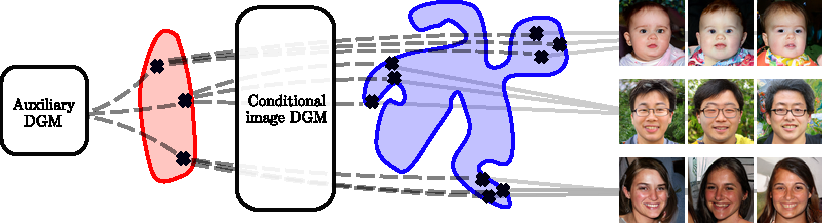
\includegraphics[width=\textwidth]{figs/2sdm/vcdm-diagram.pdf}
    \caption{Visualisation of the procedure to sample from our two-stage diffusion model. First the auxiliary DM samples a CLIP embedding, corresponding to a cross in the space of CLIP embeddings (red) in our illustration. Next, our conditional image model maps from the sampled CLIP embedding to a sampled image, visualized on the image manifold (blue). The distribution over plausible images is complex and multi-modal but becomes simpler when conditioned on a CLIP embedding. On the right we show three rows of sampled images. Within each row, all images are generated given the same CLIP embedding.}
    \label{fig:samples}
\end{figure}
We propose the solution depicted in \cref{fig:samples}. A first ``auxiliary DM'' samples vectors within an embedding space, with any vector describing a particular set of semantic characteristics of an image. The second stage, a ``conditional image DM'', takes such a vector as input and samples an image with these semantic characteristics. The vector embedding is informative, as evidenced by the fact that all images within each row on the right of \cref{fig:samples}, which are all conditioned on the same embedding, look very similar. The conditional image DM therefore inherits all the previously-described advantages of strongly-conditional DMs even though our overall generative model is unconditional (or, with the generalisation we will introduce shortly, lightly-conditional). We call the resulting model a Two-Stage Diffusion Model (2SDM).

To describe this model more precisely, we first introduce some notation. Recall that, for unconditional generation, the user does not wish to specify any input to condition on and, for the lightly-conditional setting, any such input is low-dimensional. We will condition our model on any such input in a similar way to the variable that we have been calling $\rvy$ but, to distinguish such additional conditioning input from the CLIP embeddings that we also want to condition on, we will call it $\rva$. Specifically, $\rva$ is a low-dimensional input in the lightly-conditional setting or a null variable in the unconditional setting. For the rest of \cref{sec:conditioning-on-more-improves-performance} we will use $\rvy := e_i(\rvx)$ to refer to a CLIP image embedding. To make this deterministic encoding compatible with a probabilistic generative modelling perspective, we consider a joint distribution $\pdata(\rvx, \rvy, \rva)=\pdata(\rvx, \rva)\delta_{e_i(\rvx)}(\rvy)$, where $\pdata(\rvx, \rva)$ is described by a dataset and $\delta_{e_i(\rvx)}(\rvy)$ is a Dirac conditional distribution enforcing that $\rvy$ is the CLIP embedding of $\rvx$. For the rest of this chapter all distributions denoted with $\pdata$ should be understood as marginals and/or conditionals of this joint distribution, including our target distribution $\pdata(\rvx|\rva)$. 2SDM approximates this target distribution as
%
\begin{align} \label{eq:no-a}
    \pdata(\rvx|\rva) &= \mathbb{E}_{\pdata(\rvy|\rva)} \left[ \pdata(\rvx|\rvy,\rva) \right] \\
    &\approx \mathbb{E}_{p_\phi(\rvy|\rva)} \left[ p_\theta(\rvx|\rvy,\rva) \right] % = p_{\theta,\phi}(\rvx|\rva)
\end{align}
where $p_\theta(\rvx|\rvy,\rva)$ is a conditional image DM modelling $\rvx$ given $\rvy$ and $\rva$ while $p_\phi(\rvy|\rva)$ is a second DM modelling the CLIP embeddings $\rvy$ given $\rva$. We can sample from this distribution by sampling $\rvy\sim p_\phi(\cdot|\rva)$ and then leveraging the conditional image DM to sample $\rvx \sim p_\theta(\cdot|\rvy,\rva)$ We then return $\rvx$ and make no further use of $\rvy$.
%
From now on we will call $p_\theta(\rvx|\rvy,\rva)$ the \textit{conditional image model} and $p_\phi(\rvy|\rva)$ the \textit{auxiliary model}. In our experiments the auxiliary model uses a small architecture relative to the conditional image model and so adds little extra cost.\footnote{For our ImageNet experiments, sampling from our auxiliary model takes 35ms per batch item. Sampling from our image model takes 862ms and so 2SDM has inference time only $4\%$ greater than our baselines.}


\paragraph{Auxiliary model}
Our auxiliary model is a conditional DM targeting $\pdata(\rvy|\rva)$, where $\rvy$ is a 512-dimensional CLIP embedding. Following \cref{eq:cond-diffusion-loss}, we train it by minimising
\begin{equation}
\label{eq:auxiliary-model-objective}
    \mathbb{E}_{u(\sigma)q(\rvy_\sigma|\rvy)\pdata(\rvy,\rva)} \left[ \frac{\lambda^\rvx(\sigma)}{u(\sigma)} \lvert\lvert \rvy - \hat{\rvy}_\theta(\rvy_\sigma, \rva, \sigma) \rvert\rvert_2^2 \right]
\end{equation}
where $q(\rvy_\sigma|\rvy) = \gN(\rvy_\sigma; \rvy, \sigma^2\mI)$. We use a variance-exploding diffusion process following \citet{karras2022elucidating}, and also match their diffusion process hyperparameters, including $\lambda^\rvx$ and $u(\sigma)$ (which is a continuous distribution), and use their proposed Heun sampler. We follow the architectural choice of \citet{ramesh2022hierarchical} and use a DM with a transformer architecture. It takes as input a series of 512-dimensional input tokens: an embedding of $\sigma$; an embedding of $\rva$ if this is not null; an embedding of $\rvy_\sigma$; and a learned query. These are passed through six transformer layers and then the output corresponding to the learned query token is used as the output. Like \citet{ramesh2022hierarchical}, we parameterise the DM to directly output a mean-squared error estimate of $\rvy$.
%
On AFHQ and FFHQ we find that data augmentation is helpful to prevent the auxiliary model overfitting. We perform augmentations (including rotation, flipping and color jitter) in image space and feed the augmented image through $e_i(\cdot)$ to obtain an augmented CLIP embedding. Following \citet{karras2022elucidating}, we pass a label describing the augmentation into the transformer as an additional input token so that we can condition on there being no augmentation at test-time.


\paragraph{Conditional image model}
Including the additional conditioning input $\rva$, the conditional image model's training objective is
\begin{equation}
\label{eq:conditional-image-model-objective}
    \mathbb{E}_{u(\sigma)q(\rvx_\sigma|\rvx)\pdata(\rvx,\rvy,\rva)} \left[ \frac{\lambda^\rvx(\sigma)}{u(\sigma)} \lvert\lvert \rvx - \hat{\rvx}_\theta(\rvx_\sigma, \rvy \oplus \rva, \sigma) \rvert\rvert_2^2 \right].
\end{equation}
where $\rvy \oplus \rva$ is the concatenation of $\rvy$ and $\rva$ to form a single vector which the image model is conditioned on. As with the auxiliary model, we use a variance-exploding diffusion process with the hyperparameters and Heun solver of \citet{karras2022elucidating}. For AFHQ and FFHQ, we use the U-Net architecture originally proposed by \citet{song2020score}. For ImageNet, we use the slightly larger U-Net architecture proposed by \citet{dhariwal2021diffusion}. We match the data augmentation scheme to be the same as that of \citet{karras2022elucidating} on each dataset. There are established conditional variants of both architectures~\citep{dhariwal2021diffusion,karras2022elucidating} that add a learned linear projection to the embedding of the noise standard deviation $\sigma$.  We use the same technique to incorporate the concatenated conditioning inputs $\rvy\oplus\rva$.

\subsection{Two-stage diffusion improves over standard diffusion} \label{sec:2sdm-experiments}


\begin{table}[t]
\centering
\small
\caption{Comparison of a standard diffusion model (EDM) with our two-stage approach (2SDM) on a suite of image-generation metrics. Best performance for each metric and dataset is shown in bold. Higher is better for metrics marked $\uparrow$; lower is better for $\downarrow$. Results reported for EDM on FFHQ and AFHQ are computed with the pretrained checkpoints released by \citet{karras2022elucidating}. Results reported for 2SDM on FFHQ are with finetuning from this pretrained checkpoint. All others are trained from scratch.}
\begin{tabular}{lcccccccccc}
\toprule
 \multirow{2}{*}{Dataset} & \multirow{2}{*}{Method} & \multirow{2}{*}{\shortstack{Inception\\Score $\uparrow$}} & \multirow{2}{*}{Precision $\uparrow$} & \multirow{2}{*}{Recall $\uparrow$} & \multirow{2}{*}{FID $\downarrow$} & \multirow{2}{*}{sFID $\downarrow$} \\
 & & & & & & \\
\midrule
\multirow{2}{*}{AFHQ-64} & 2SDM & $\mathbf{10.00}$ & $\mathbf{0.844}$ & $\mathbf{0.619}$ & $\mathbf{1.56}$ & $13.7$ \\
 & EDM & $8.91$ & $0.752$ & $0.614$ & $2.04$ & $13.7$ \\
\midrule
\multirow{2}{*}{FFHQ-64} & 2SDM & $\mathbf{3.47}$ & $\mathbf{0.721}$ & $\mathbf{0.697}$ & $\mathbf{2.32}$ & $4.98$ & \\
 & EDM & $3.33$ & $0.697$ & $0.569$ & $2.46$ & $\mathbf{4.90}$ \\
\midrule
\multirow{2}{*}{\shortstack[l]{Class-cond. \\ ImageNet-64}} & 2SDM & $\mathbf{17.3}$ & $\mathbf{0.541}$ & $\mathbf{0.573}$ & $\mathbf{17.4}$ & $\mathbf{4.63}$ \\
 & EDM & $13.6$ & $0.530$ & $0.532$ & $25.4$ & $6.50$ \\
\midrule
\multirow{2}{*}{\shortstack[l]{Uncond. \\ ImageNet-64}} & 2SDM & $\mathbf{15.6}$ & $\mathbf{0.614}$ & $\mathbf{0.526}$ & $\mathbf{21.0}$ & $\mathbf{5.59}$ \\
 & EDM & $11.3$ & $0.523$ & $0.524$ & $35.1$ & $9.14$ \\
 \midrule
\multirow{2}{*}{\shortstack[l]{Class-cond. \\ latent \\ ImageNet-256}} & 2SDM & $\mathbf{52.1}$ & $\mathbf{0.590}$ & $0.603$ & $\mathbf{24.3}$ & $\mathbf{7.36}$ \\
 & EDM & $40.4$ & $0.532$ & $\mathbf{0.610}$ & $34.2$ & $9.59$ \\
\end{tabular}
\label{tab:2sdm-many-metrics}
\end{table}

\paragraph{Experimental setup and results overview}

We perform experiments in five settings: unconditional AFHQ modelling at $64\times64$ resolution~\citep{choi2020stargan}; unconditional FFHQ modelling at $64\times64$ resolution~\citep{karras2018style}; class-conditional ImageNet modelling at $64\times64$ resolution~\citep{deng2009imagenet}; unconditional ImageNet modelling at $64\times64$ resolution; and finally class-conditional latent ImageNet modelling in which we model a compressed $32\times32\times4$ representation of a $256\times256$ image as we will describe shortly. In every setting, we compare against EDM~\citep{karras2022elucidating}, a standard DM directly modelling $\pdata(\rvx|\rva)$, with an identical architecture to 2SDM's conditional image model. We also match the training compute of our conditional image model with that of EDM in every case. Auxiliary models for each setting are trained for one day on a single V100 GPU so add little additional cost. We report the metrics achieved by each of EDM and 2SDM on each setting in \cref{tab:2sdm-many-metrics} before giving more detail and analysis of the models in each setting. The Inception Score~\citep{salimans2016improved,barratt2018note} in \cref{tab:2sdm-many-metrics} measures the diversity of the output from an image classifier when run on sampled images. The Precision and Recall metrics~\citep{kynkaanniemi2019improved} estimate, roughly speaking, the proportion of generated images that lie on the data manifold (Precision) and the proportion of dataset images that can be found within the manifold of generated images (Recall). The FID approximates the distance between the distribution of embeddings of dataset images and that of embeddings of generated images. The sFID is similar but uses an embedding with more spatial information. 2SDM outperforms EDM on 22 of the 25 metric-dataset combinations, and is outperformed on only 2.


\begin{figure*}[t]
    \centering
    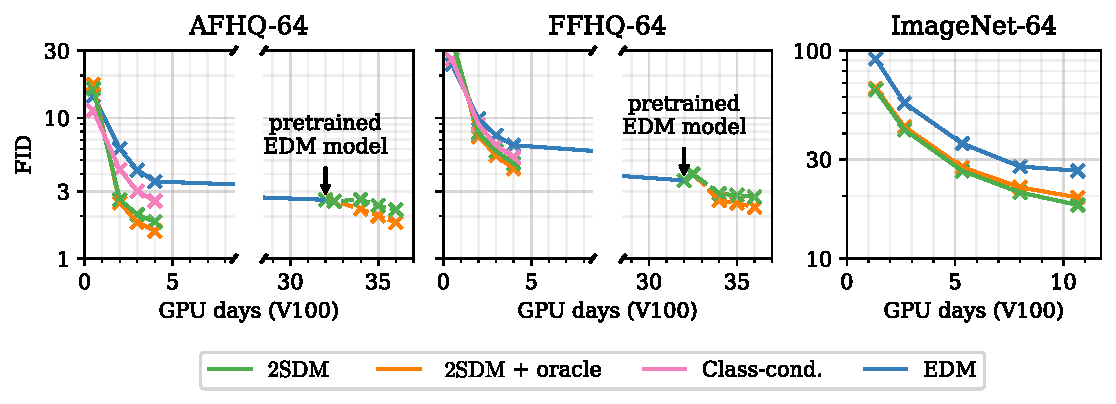
\includegraphics[width=\textwidth]{figs/2sdm/cond-results-1.pdf}
    \caption{FID throughout training for our method and baselines on AFHQ, FFHQ, and class-conditional ImageNet-64. We show results for each method trained from scratch and, on AFHQ and FFHQ, for finetuning a pretrained EDM model (which was trained for the equivalent of 32 GPU days). 2SDM quickly outperforms EDM when trained from scratch and quickly improves on the pretrained model when used for finetuning.}
    \label{fig:fid_vs_training}
\end{figure*}


\paragraph{Details and analysis for AFHQ, FFHQ, and ImageNet-64}
On AFHQ and FFHQ, we match the EDM parameters to those of \citet{karras2022elucidating}. On ImageNet-64, we have a smaller training budget and so decrease the batch size to 128 and the learning rate to $1\times10^{-4}$. For simplicity we match 2SDM to use the same learning rate and batch size. \cref{fig:fid_vs_training} reports the FID throughout the training of the conditional image diffusion model (or image DM baseline) for AFHQ, FFHQ, and class-conditional ImageNet-64.\footnote{Each FID in \cref{fig:fid_vs_training} is estimated using $20\,000$ images, each sampled with the SDE solver proposed by \citet{karras2022elucidating} using 40 steps, $S_\text{churn}=50$, $S_\text{noise}=1.007$, and other parameters set to their default values. Our other reported FID scores use $50\,000$ samples, as is standard, and the same sampler hyperparameters.}  We consider training the conditional image model from scratch (for up to 4 GPU days on AFHQ and FFHQ, or up to 11 GPU days on ImageNet-64), and see that it improves upon our EDM baseline for any training budgets over 1-2 GPU days. For AFHQ, this improvement is so substantial that 2SDM's FID after two GPU days is better than that of the pretrained EDM model released by \citet{karras2022elucidating}, which was trained for the equivalent of 32 V100 GPU days. In addition to training from scratch, on AFHQ and FFHQ we consider initializing 2SDM's training from the pretrained EDM checkpoints. To do so, we simply add a learnable linear projection of the CLIP embedding and initialize its weights to zero. We see that this allows for a fast and significant improvement in FID over the baseline in each case. We note, though, that training 2SDM from scratch for 4 GPU days outperforms 4 GPU days of finetuning on AFHQ and so recommend training 2SDM from scratch when sufficient compute is available.

\Cref{fig:fid_vs_training} also compares against ``2SDM + oracle'', which is a supposed upper bound on 2SDM's performance given by sampling a CLIP image embedding from an oracle (in practice, the dataset) and then using 2SDM's conditional image model to sample an image conditioned on it. It therefore describes the performance that 2SDM would achieve with a perfect auxiliary model. On AFHQ-64, 2SDM with an oracle achieves a FID $56\%$ lower than EDM. Without an oracle, 2SDM still achieves a FID $48\%$ lower than 2SDM. We therefore say that 2SDM yields an improvement $87\%$ as large as can be gleaned by using a purely conditional DM. Similarly for FFHQ, 2SDM obtains an improvement $81\%$ as large as is possible with a purely conditional DM.\footnote{Our calculation of these numbers is as follows. On AFHQ-64, 2SDM with an oracle achieved a FID of $1.57$, a $56\%$ improvement on the FID of $3.53$ achieved with EDM. 2SDM without an oracle achieved a FID of $1.83$, a $48\%$ improvement on $3.53$. This is $87\%$ as large as the improvement achieved with an oracle. Similarly on FFHQ-64, 2SDM with an oracle achieved a FID of $4.35$, a $32\%$ improvement on the FID of $6.39$ achieved with EDM. 2SDM without an oracle achieved a FID of $4.73$, a $26\%$ improvement on $6.39$. This is $81\%$ as large as the improvement achieved with an oracle.} We can therefore say that our cheaply-trained auxiliary model is good enough to allow us to capture the majority of the benefits of conditional generation for the unconditional generation task. Intriguingly,
 on ImageNet-64, 2SDM achieves better FID \textit{without} an oracle. This suggests that imperfections in the distribution
learned by the auxiliary model improve the visual quality of the generated images. We observed this trend consistently on ImageNet, and believe that characterising exactly when and why it occurs is an intriguing direction for future work.

Finally, \cref{fig:fid_vs_training} also compares against ``Class-cond'', which is an ablation of 2SDM in which we replace the CLIP embedding $\rvy$ with a single discrete label obtained by K-means clustering of the CLIP embedding (as on the right of \cref{fig:fid-vs-ncomp}). For unconditional generation tasks, we can then replace our auxiliary model with a simple categorical distribution modelling $\pdata(\rvy|\rva)=\pdata(\rvy)$ similarly to \citet{hu2022self}, simplifying the generative procedure. We see that this baseline is outperformed by 2SDM, justifying our choice to use a continuous $\mathbf{y}$.

\begin{figure}[t]
    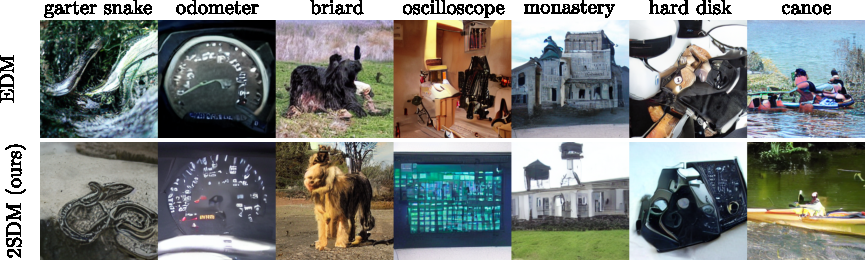
\includegraphics[width=\textwidth]{figs/2sdm/2SDM-main-fig.pdf}
    \caption{Comparison of class-conditional ImageNet-256 samples from our two-stage diffusion model, 2SDM, and from a diffusion model baseline, EDM~\citep{karras2022elucidating}. Both are trained for 12 GPU days. Samples within the same column are generated with the same random seed and class label.}
    \label{fig:latent-imagenet-samples}
\end{figure}

\paragraph{Details and analysis for ImageNet-256}
We combine 2SDM and the latent diffusion modelling framework~\citep{rombach2022high} on the ImageNet-256 dataset as follows. We take the pretrained encoder and decoder of the Stable Diffusion auto-encoder released by \citet{rombach2022high}. We feed $256\times256\times3$ dataset images through the VAE encoder to create $64\times64\times4$ tensors, which we use as the training targets $\rvx$ for our conditional image model. The training targets for the CLIP embeddings $\rvy$ are created by embedding the $256\times256\times3$ images with the standard CLIP image embedder. We use the ImageNet class labels as additional inputs $\rva$. At test time, we take $\rva$ as an input; we then sample $\rvy$ given $\rva$ from our auxiliary model; we then sample $\rvx$ given $\rvy$ and $\rva$ from our conditional image model; we finally use the Stable Diffusion VAE decoder to produce an image given $\rvx$. Samples from this version of 2SDM, as well as our EDM baseline operating in the same latent space, are shown in \cref{fig:latent-imagenet-samples}. While the compute used for each (12 GPU days) is far from that of the state-of-the-art for this dataset, the samples from 2SDM are noticeably better, supporting the FID scores in \cref{tab:2sdm-many-metrics}.

\paragraph{Comparison of relative improvements between tasks}
In terms of FID, and for the networks trained from scratch and matched for training compute, the percentage improvement of 2SDM over EDM is $48.2\%$ on AFHQ-64; $26.0\%$ on FFHQ-64; $31.5\%$ on class-conditional ImageNet-64; $40.2\%$ on unconditional ImageNet-64; and $28.9\%$ on class-conditional ImageNet-256. While these are all substantial improvements, we point out two comparisons in particular. 

First, the gain from using 2SDM on unconditional ImageNet-64 ($40.2\%$) is greater than that on class-conditional modelling of the same dataset ($31.5\%$). This supports our argument that two-stage diffusion techniques like 2SDM can have even greater impact in unconditional (or lightly-conditional) generation than in the text-conditional (or strongly-conditional) setting in which they were originally introduced with unCLIP~\citep{ramesh2022hierarchical}.  Noting that the class label already contains some of the information stored in a CLIP embedding, this finding also fits with our discussion of the effects of conditioning in \cref{sec:2sdm-cond-vs-uncond-dgms}. In particular, our discussion in \cref{sec:2sdm-cond-vs-uncond-dgms} suggests that the performance of an image model conditioned on just a class label (EDM on class-cond. ImageNet) should be somewhere in between that of an unconditional image model (EDM on uncond. ImageNet) and that of a CLIP-conditional image model (2SDM, assuming the auxiliary model is good), and we find that this is true.

Second, the $28.9\%$ improvement in performance for the latent diffusion model on ImageNet-256 is only slightly less than the $31.5\%$ improvement for pixel-space diffusion on class-conditional ImageNet-64. This supports that the 2SDM approach of conditioning on high-level but low-dimensional embeddings is readily combined with the widely-used latent diffusion framework, which models the data via a relatively high-dimensional representation.

\paragraph{Inference speed}
Sampling from 2SDM does impose a small additional cost relative to EDM, since we must begin by sampling from the auxiliary model. In all experiments, when we use 40 diffusion steps, sampling from our auxiliary model takes 8.8s with batch size 256. This corresponds to 35ms per batch item. Our conditional image model and our EDM baseline use identical architectures (other than the projection of $\rvy$) and we could not detect a difference between their sampling times which were 862ms per batch item on our ImageNet architecture and 789ms per batch item on our AFHQ and FFHQ architecture. This means that the increase in time due to using 2SDM instead of EDM is less than $4\%$. Furthermore, we can negate this increase by using two less sampling steps for the conditional image model. We show in \cref{supp:conditional-diffusion} that this lets us make 2SDM faster than EDM with almost no effect on sample quality.


\subsection{Perspectives on two-stage diffusion}
\textbf{UnCLIP} \label{sec:unclip}
UnCLIP~\citep{ramesh2022hierarchical} uses the following text-to-image procedure: given a text prompt, it is embedded by a CLIP text embedder. A diffusion model then samples a plausible CLIP image embedding with high cosine similarity to this text image embedding. Finally, a conditional image diffusion model samples an image conditioned on CLIP image embedding and text prompt. This is described as ``inverting'' the CLIP embedder framework to map from image to text, hence the name unCLIP. Given our discssion of the benefits of conditioning the diffusion model on as much information as possible, it makes sense that unCLIP provides a benefit as long as the combination of text and CLIP embedding contains ``more'' information than the text prompt alone, which will always be the case. They also imply that the disparity is even larger if we compare the CLIP-conditional generative model with an unconditional generative model  (i.e. one conditioned on zero bits of information). The unCLIP approach can therefore be expected to provide larger benefits for unconditional (or lightly-conditional) generation than for the text-conditional setting in which it was developed. This is supported by our findings with 2SDM which show bigger benefits over EDM for unconditional generation than for class-conditional generation.

\textbf{Intermediate variables in diffusion models}~
 Our work takes inspiration from \citet{weilbach2023graphically}, % who use diffusion models to perform approximate inference in graphical models. They 
who show improved performance in various approximate inference settings by modelling problem-specific auxiliary variables (like $\rvy$) in addition to the variables of interest ($\rvx$) and observed variables ($\rva$). We apply these techniques to the image domain and incorporate pretrained CLIP embedders to obtain auxiliary variables. 

\textbf{Latent diffusion}~
2SDM also relates to methods which perform diffusion in a learned latent space~\citep{rombach2022high}: our auxiliary model $p_\phi(\rvy|\rva)$ is analogous to a ``prior'' in a latent space and our conditional image model $p_\theta(\rvx|\rva,\rvy)$ to a ``decoder'' Such methods typically use a near-deterministic decoder and so their latent variables must summarize all information about the image. Our conditional DM decoder, on the other hand, is a DM that will function reasonably however little information is stored in $\rvy$. This means that 2SDM provides an additional degree of freedom in terms of what to store. Furthermore, as we showed in \cref{sec:2sdm-experiments}, 2SDM can be fruitfully combined with latent diffusion.

\textbf{Self-supervised representations}~
\citet{bao2022conditional,hu2022self} both use self-supervised learning to obtain auxiliary variables and then training a diffusion model $p(\rvx|\rva)$. However, they do not model $\rva$ and therefore are not able to sample $\rvx$ without an oracle that can provide $\rva$. Their success when given an oracle, however, provides reason to believe that our approach is likely to yield benefits even if the embedder that produces $\rva$ is obtained through self-supervised learning and without access to additional (or multi-modal) data as our CLIP embedder was trained with.

\textbf{Integrating additional data}~
Our method can be understood as a means to leverage the ``world knowledge'' inside a CLIP embedder for improved performance on the image generation task. Another way in which additional knowledge, or data, could be leveraged is by training a multi-headed diffusion model which simultaneously approximates the score function and makes predictions of side information like class labels. \citet{deja2023learning} propose a method for doing so but do not demonstrate improved performance on the unconditional generation task.

\subsection{Final discussion of two-stage diffusion}
In this section we have demonstrated that conditional DMs can outperform unconditional DMs in terms of sample realism in the image domain, and that we can leverage this insight to build improved unconditional and lightly-conditional DGMs. This provides motivation for our work on conditional generation in addition to the new systems that are enabled by the capability to do conditional generation. 

We note, though, that a massive unexplored design space remains after the results we have presented on 2SDM. For pedagogical purposes we intentionally kept 2SDM simple, using known diffusion architectures and objectives. It is likely that optimising these design choices for the lightly-conditional 2SDM use-case would improve performance. In addition, there are almost certainly more useful quantities that we could condition on than CLIP embeddings. 
\citet{bao2022conditional,hu2022self} have shown that self-supervised learning techniques provide a promising avenue for obtaining useful ``latent'' representations. Exactly the properties that an embedding should have to be beneficial for techiques like 2SDM is another open question that is ripe for future work to tackle. Such a line of work may also fix one limitation of 2SDM, namely that it relies on the availability of a pretrained CLIP embedder. While this is freely available for natural images, it could be a barrier to other applications. Improvements may also be gleaned by conditioning on multiple quantities, or ``chaining'' a series of conditional DMs together. An alternative direction is to simplify 2SDM's architecture by, for example, learning a single diffusion model over the joint space of $\rvx$ and $\rvy$ instead of generating them sequentially.

\section{Other methods for conditional sampling} \label{sec:other-methods-for-conditional-sampling}
So far we have described how diffusion models can be trained explicitly as conditional models, and the technique we described for doing so will form the foundation of this thesis. Another class of methods, though, which we will use in \cref{ch:tddm}, make it possible to draw conditional samples from \textit{unconditional} diffusion models. In particular, in this section we will describe the replacement method, reconstruction guidance, and classifier guidance~\citep{song2020score,kadkhodaie2020solving,mittal2021symbolic,ho2022video}. We will finally discuss classifier-free guidance, which can build on these techniques to sometimes improve the sample quality attainable with a conditional diffusion model.

\subsection{Replacement method}
We first describe a method proposed by \citet{song2020score} to use an unconditional diffusion model for imputation; i.e. to sample the values of a subset of the dimensions of $\rvx$ conditioned on the values of the other dimensions. Recalling our notation from \cref{ch:introduction}, let $\gY$ be a list containing the indices of any dimension with observed values and let $\rvy = \rvx[\gY]$ be their observed values.
Similarly, let $\rvx_t[\gY]$ to denote all the values in $\rvx_t$ corresponding to observed values in $\rvx$.
\citet{song2020score} suggest modifying $\rvx_t[\gY]$ at each integration step while sampling from the reverse SDE. In particular, they modify the values of $\rvx_t$ at indices $\gY$ by replacing them with samples from $q(\rvx_t[\gY] ~|~ \rvx[\gY] )$, i.e. with the observed values plus time-dependent noise. This method is sometimes referred to as the ``replacement method'' as it simply continuously replaces some dimensions of $\rvx_t$ with new values that tend towards their observed values as $t$ tends to zero.

\subsection{Conditioning on any linear projection}
The replacement method described above is applicable more generally in that, as well as being used to condition on the values of any subset of the dimensions in $\rvx$, it can be used to condition on the value of any linear projections of $\rvx$. That is, given an unconditional diffusion model that predicts the score function $\rvs_\theta(\rvx_t, t) \approx \nabla_{\rvx_t} \log q(\rvx_t)$, we can draw samples from an approximation of $\pdata(\rvx|\rvy)$ where $\rvy:=\mA\rvx$ for any projection matrix $\mA \in \mathbb{R}^{m \times n}$ with number of columns $m$ matching the dimensionality of $\rvy$ and number of columns $n$ matching the dimensionality of $\rvx$.

To do so, \citet{song2020score} point out that it is always possible to rotate the data given $\mA$ such that some dimensions are fully observed and the remainder are fully unobserved. At this point, the replacement method described previously can be used. To perform the rotation, we will assume that the rows of $\mA$ are of unit magnitude and are orthogonal to eachother.\footnote{We can do so without loss of generality since it is possible to transform any $\mA$ to meet these conditions without changing the information stored in $\rvy$ using the Gram-Schmidt process.} We then add more basis vectors to create a rotation matrix $\mR \in \mathbb{R}^{m \times m}$ such that its first $m$ rows are the rows of $\mA$. We can then transform $\rvx$ into $\hat{\rvx} := \mR \rvx$. The first $m$ dimensions of $\hat{\rvx}$ have observed values $\rvy := \mA\rvx$ and the remaining $n-m$ are to be sampled with the diffusion model. This means that we can use the replacement method, as described in the previous method, to sample $\hat{\rvx}$ as long as we can compute the score $\nabla_{\hat{\rvx}_t} \log q(\hat{\rvx}_t)$. As shown by \citet{song2020score}, this is simple to compute as $\nabla_{\hat{\rvx}_t} \log q(\hat{\rvx}_t) = \mR \nabla_{\rvx_t} \log q(\rvx_t) \approx \mR \rvs_\theta(\rvx_t, t) = \mR \rvs_\theta(\mR^\top \hat{\rvx}_t, t)$. Once we have sampled $\hat{\rvx}$ given $\rvy$, we can transform it into the original data space as $\rvx = \mR^\top \hat{\rvx}$.

\subsection{Reconstruction guidance} \label{sec:reconstruction-guidance}
\citet{ho2022video} point out that the replacement method is not a perfect approximation of the desired conditional distribution because it estimates the score function as $\nabla_{\rvx_t} \log q(\rvx_t)$ instead of as $\nabla_{\rvx_t} \log q(\rvx_t~|~\rvx[\gY])$. While $\rvx_t$ does contain some information about $\rvx[\gY]$ thanks to $\rvx_t[\gY]$ being sampled from $q(\cdot ~|~ \rvx[\gY])$, there is still information lost due to the noise in $q(\rvx_t[\gY] ~|~ \rvx[\gY])$ and so these two score functions are not the same. \citet{ho2022video} derive an approximation by breaking the desired conditional score function into two terms as
\begin{align}
    \nabla_{\rvx_t} \log q(\rvx_t~|~\rvx[\gY]) &= \nabla_{\rvx_t} \log \frac{q(\rvx_t, \rvx[\gY])}{q(\rvx[\gY])}\\
    &= \nabla_{\rvx_t} \log \left( q(\rvx_t) q(\rvx[\gY]~|~\rvx_t) \right) - \underbrace{\nabla_{\rvx_t} \log q(\rvx[\gY])}_{=0} \\
    &= \underbrace{\nabla_{\rvx_t} \log q(\rvx_t)}_\text{estimated by diffusion model} + \underbrace{\nabla_{\rvx_t} \log q(\rvx[\gY]~|~\rvx_t)}_\text{intractable}. \label{eq:approx-score-function-recon-guidance}
\end{align}
The final term of \cref{eq:approx-score-function-recon-guidance} is unfortunately intractable, but \citet{ho2022video} suggest approximating it by assuming that $q(\rvx[\gY]~|~\rvx_t)$ is a Gaussian whose mean is the neural network's prediction of $\rvx$ for observed dimensions, $\hat{\rvx}_\theta(\rvx_t, t)[\gY]$, and with element-wise standard deviation $\sigma(t) / \alpha(t)$. This leads to the score function
\begin{align}
    \nabla_{\rvx_t} \log q(\rvx[\gY]~|~\rvx_t) &\approx \nabla_{\rvx_t} \log \gN( \rvx[\gY]; \hat{\rvx}_\theta(\rvx_t, t)[\gY], \frac{\sigma(t)^2}{\alpha(t)^2} \mI ) \\
    &= -\frac{\alpha(t)^2}{2\sigma(t)^2} \nabla_{\rvx_t} || \rvx[\gY] - \hat{\rvx}_\theta(\rvx_t, t)[\gY] ||_2^2.
\end{align}
\citet{ho2022video} suggest adding a scaling factor $w$ to allow for controllability of how ``strongly conditioned'' the output is on $\rvy$ and so finally estimate the score function as 
\begin{align}
    \nabla_{\rvx_t} \log q(\rvx_t~|~\rvx[\gY]) &= \nabla_{\rvx_t} \log q(\rvx_t) - \frac{w \cdot \alpha(t)^2}{2\sigma(t)^2} \nabla_{\rvx_t} || \rvx[\gY] - \hat{\rvx}_\theta(\rvx_t, t)[\gY] ||_2^2 . \label{eq:recon-guidance-score-function}
\end{align}
Other than using this updated score function to take each step, reconstruction guidance has all other steps identical to the replacement method described above. Note that computing the second term in \cref{eq:recon-guidance-score-function} requires differentiating through the neural network, so performing reconstruction guidance makes sampling more computationally expensive than using the replacement method. 

\subsection{Classifier guidance}
Classifier guidance~\citep{song2020score} applies when the conditioning information is a discrete label. It enables conditional sampling from a unconditional diffusion model, but does require one model specifically trained for the conditioning task: a classifier $p_\theta(\rvy|\rvx_t) \approx q(\rvy|\rvx_t)$ that estimates the probability of the discrete label $\rvy$ given noisy data $\rvx_t$. For e.g. an image diffusion model, this classifier might have a similar architecture to a standard image classifier but it should take noisy images as input and additionally should receive the timestep describing how noisy the input image is. We can use this if we decompose the conditional score function as
\begin{align}
    \nabla_{\rvx_t} \log q(\rvx_t|\rvy) &= \nabla_{\rvx_t} \log \frac{q(\rvx_t)q(\rvy|\rvx_t)}{q(\rvy)} \label{eq:cg-derivation-line1} \\
    &= \nabla_{\rvx_t} \log \left( q(\rvx_t) q(\rvy|\rvx_t) \right) - \underbrace{\nabla_{\rvx_t} \log q(\rvy)}_{=0}  \label{eq:cg-derivation-line2} \\
    &= \nabla_{\rvx_t} \log q(\rvx_t) + \nabla_{\rvx_t} \log q(\rvy|\rvx_t)  \label{eq:cg-derivation-line3}
\end{align}
where \cref{eq:cg-derivation-line2} follows from \cref{eq:cg-derivation-line1} because the denominator has no dependence on $\rvx_t$. We can therefore write the conditional score function as the sum of the unconditional score function and $\log \nabla_{\rvx_t} q(\rvy|\rvx_t)$. The unconditional score function is estimated by our unconditional diffusion model and we can estimate $\log \nabla_{\rvx_t} q(\rvy|\rvx_t)$ with the gradient of our classification probability with respect to $\rvx_t$:
\begin{align}
    \nabla_{\rvx_t} \log q(\rvx_t|\rvy) \approx \rvs_\theta(\rvx_t, t) + \nabla_{\rvx_t} p_\theta(\rvy|\rvx_t).
\end{align}
Note that this score function requires evaluating and backpropagating through the classifier, so using classifier guidance can be slower than using a trained conditional diffusion model. Finally, a generalisation of classifier guidance is to modify the score with a hyperparameter $\alpha \geq 0$:
\begin{align}
    \nabla_{\rvx_t} \log q(\rvx_t|\rvy) \approx \rvs_\theta(\rvx_t, t) + \alpha \nabla_{\rvx_t} p_\theta(\rvy|\rvx_t). \label{eq:cg-score-function}
\end{align}
If $\alpha$ is zero, this corresponds to the unconditional score function and if $\alpha$ is one this approximates the standard conditional score function. In practice $\alpha$ is often set to be between zero and one or to be greater than one~\citep{ho2022classifier,meng2022distillation}. While these do not lead the samples to come from any easily-described distribution, setting $\alpha$ to be between zero and one can be thought of as drawing samples from a distribution that is interpolated between the unconditional and the conditional distribution. Setting $\alpha$ to be greater than one leads to samples being ``even more'' dependent on $\rvy$ than in the true conditional distribution. Large values of $\alpha$ are also associated with samples being less diverse, as the distribution over $\rvx$ becomes tightly peaked around the values that make $\rvy$ the most plausible, and improved sample quality~\citep{ho2022classifier}.

\paragraph{Classifier-free guidance}
While the last few conditional generation methods we have looked at - the replacement method, reconstruction guidance, and classifier guidance - have all been designed for use with an unconditional diffusion model, classifier-free guidance (CFG)~\citep{ho2022classifier} relies on having a trained conditional diffusion model of the kind described earlier in this chapter. It gets is name from the fact that it requires no separately-trained classifier but still has the same flexibility as classifier guidance, in that it has the same hyperparameter $\alpha$ controlling the ``strength'' of the conditioning.

To use classifier-free guidance we require both a conditional score function $\rvs_\theta(\rvx_t, \rvy, t)$ and an unconditional score function $\rvs_\theta(\rvx_t, t)$. The unconditional score function is often parameterised with the same neural network as the conditional score function into which a null variable is input in place of $\rvy$. Rearranging \cref{eq:cg-derivation-line3}, which breaks the conditional score function into the sum of the unconditional score function and the gradient of $\log q(\rvy|\rvx_t)$, we can write this gradient as
\begin{align}
    \nabla_{\rvx_t} \log q(\rvy|\rvx_t) &= \nabla_{\rvx_t} \log q(\rvx_t|\rvy) - \nabla_{\rvx_t} \log q(\rvx_t) \\
    &\approx \rvs_\theta(\rvx_t, \rvy, t) - \rvs_\theta(\rvx_t, t).
\end{align}
We can use this approximation of $\nabla_{\rvx_t} \log q(\rvy|\rvx_t)$ inside the classifier guidance equation in \cref{eq:cg-score-function} instead of using the gradients of a trained classifier. Doing so gives the classifier-free guidance score function
\begin{align}
    \nabla_{\rvx_t} \log q(\rvx_t|\rvy) &\approx \rvs_\theta(\rvx_t, t) + \alpha \left( \rvs_\theta(\rvx_t, \rvy, t) - \rvs_\theta(\rvx_t, t) \right). \label{eq:cfg-score-function}
\end{align}
Similarly to classifier guidance, this becomes the unconditional score function or conditional score function when $\alpha$ is zero or one, but in practice larger values of $\alpha$ are often used. The image samples shown in \cref{fig:dalle-3-samples,fig:emu-edit-samples} both rely on classifier-free guidance with $\alpha > 1$. 

In the remainder of this thesis we will not use classifier-free guidance~\citep{ho2022classifier} because, for any $\alpha \neq 1$, it prevents the generated samples from targeting the desired conditional distribution. Nevertheless, much of the work we present may be possible to combine with classifier-free guidance with $\alpha>1$ in order to produce more visually impressive results.
